\documentclass{article}
    \usepackage{amsthm, amsmath}
    \usepackage{xeCJK}
    \usepackage{algorithm}
    \usepackage{algorithmicx}
    \usepackage{algpseudocode}
    \usepackage{hyperref}
    \usepackage{listings}
    
    \title{编译原理: PA1-B}
    \author{娄晨耀, 2016011343}
    \date{}
    
    
    \theoremstyle{plain}
    \newtheorem{thm}{Theorem}
    
    \theoremstyle{definition}
    \newtheorem{alg}{Algorithm}
    
    
    \begin{document}
    \maketitle
    
    \section{实现需求}

    首先理解了parse的实现,然后根据文档描述加入错误恢复功能。

    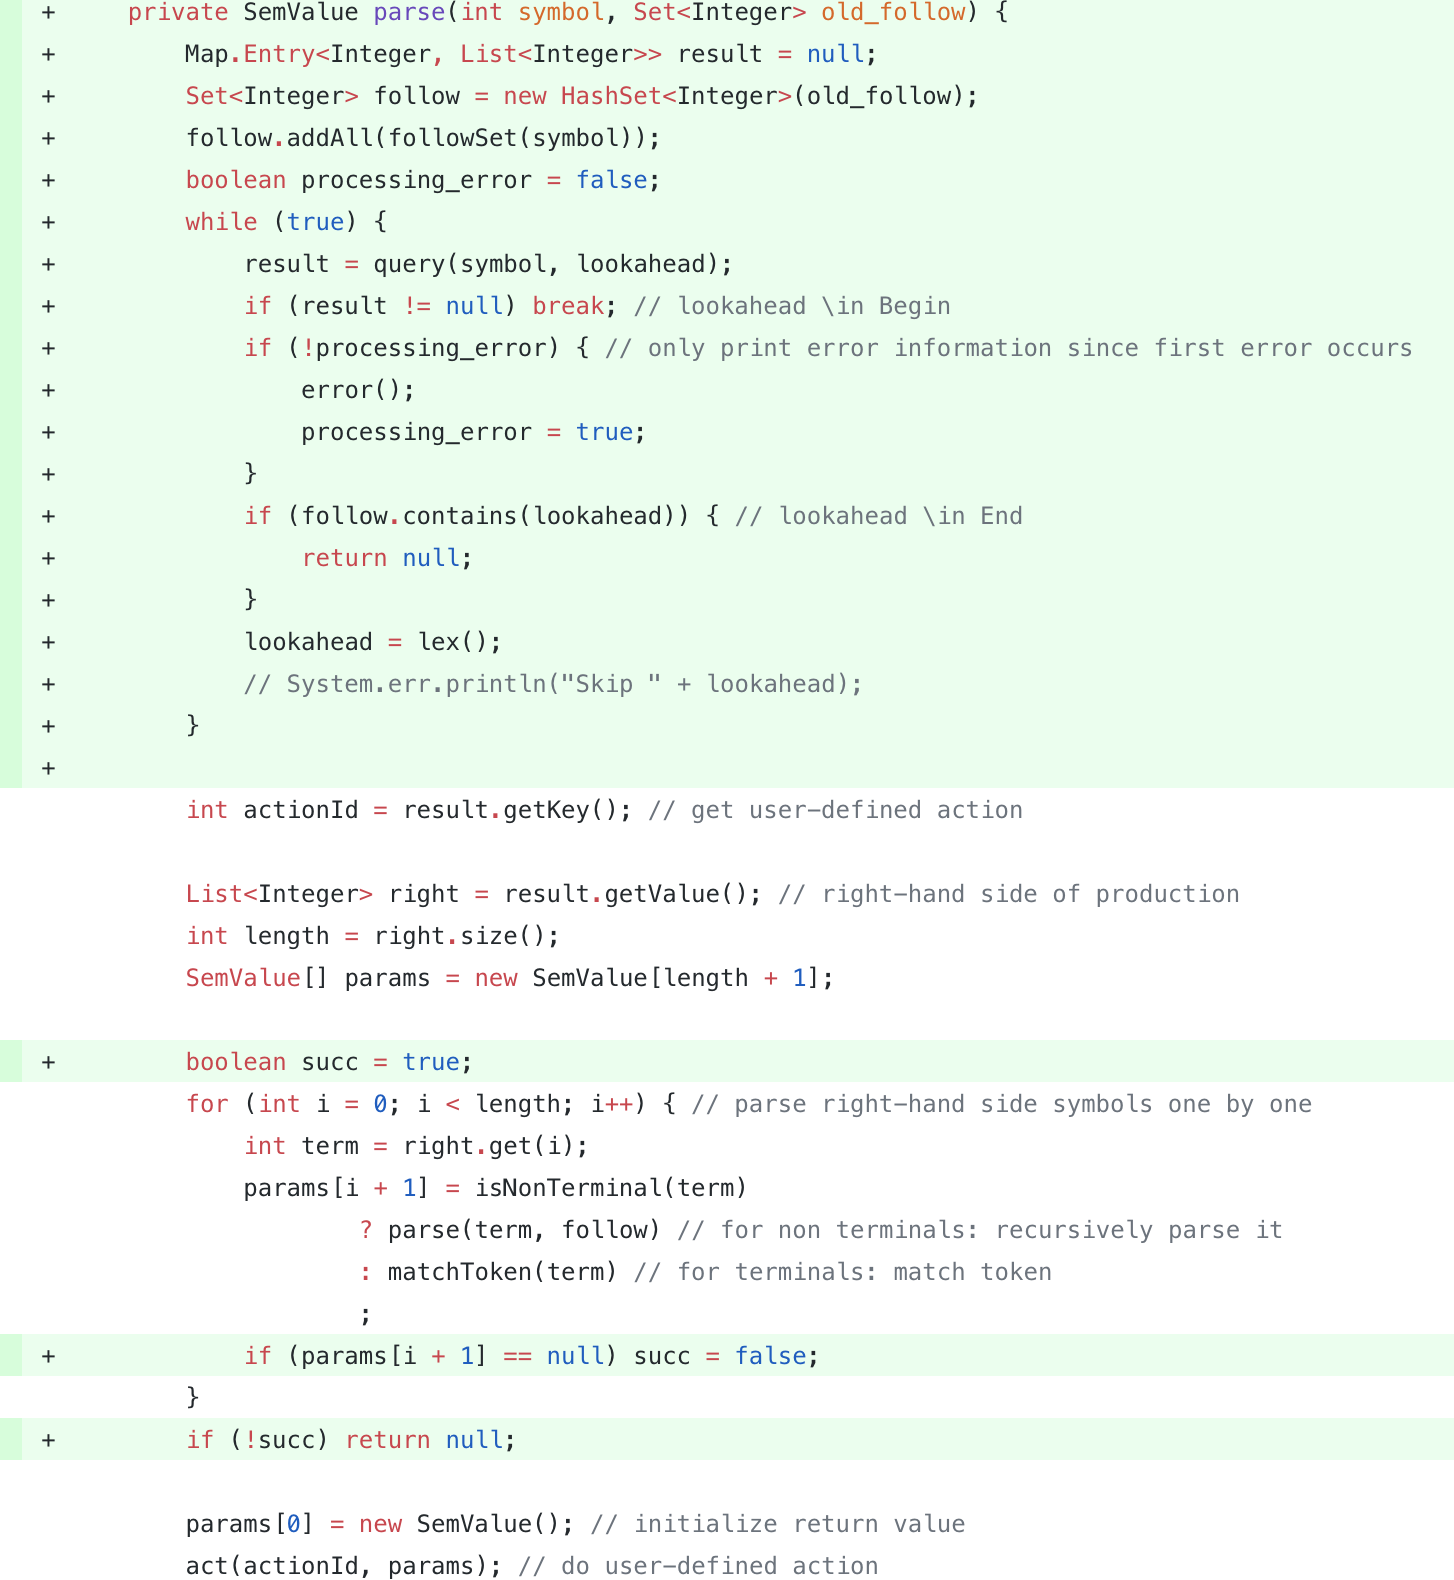
\includegraphics[width=5in]{parse.png}

    经过热心群友Harry Chen 等人的解释,我理解了如果出现错误再尝试生成合理的语法树是一件不合理的事情。但是为了尽量多的提示错误,我们如果解析错误后依然继续解析。

    另一个遇到的问题是,当我们决定跳过一个token后,如果没有恢复成功,再接下来的token如果仍要跳过我们就不需要报错了。这个听上去也很合理。

    下一步就是增加新特性,部分语法特性实现和PA-1A 类似,就不在赘述。下面只提一些不一样的地方。

    \subsection{转换之前语法为LL(1)}

    以串行卫士语句为例:

    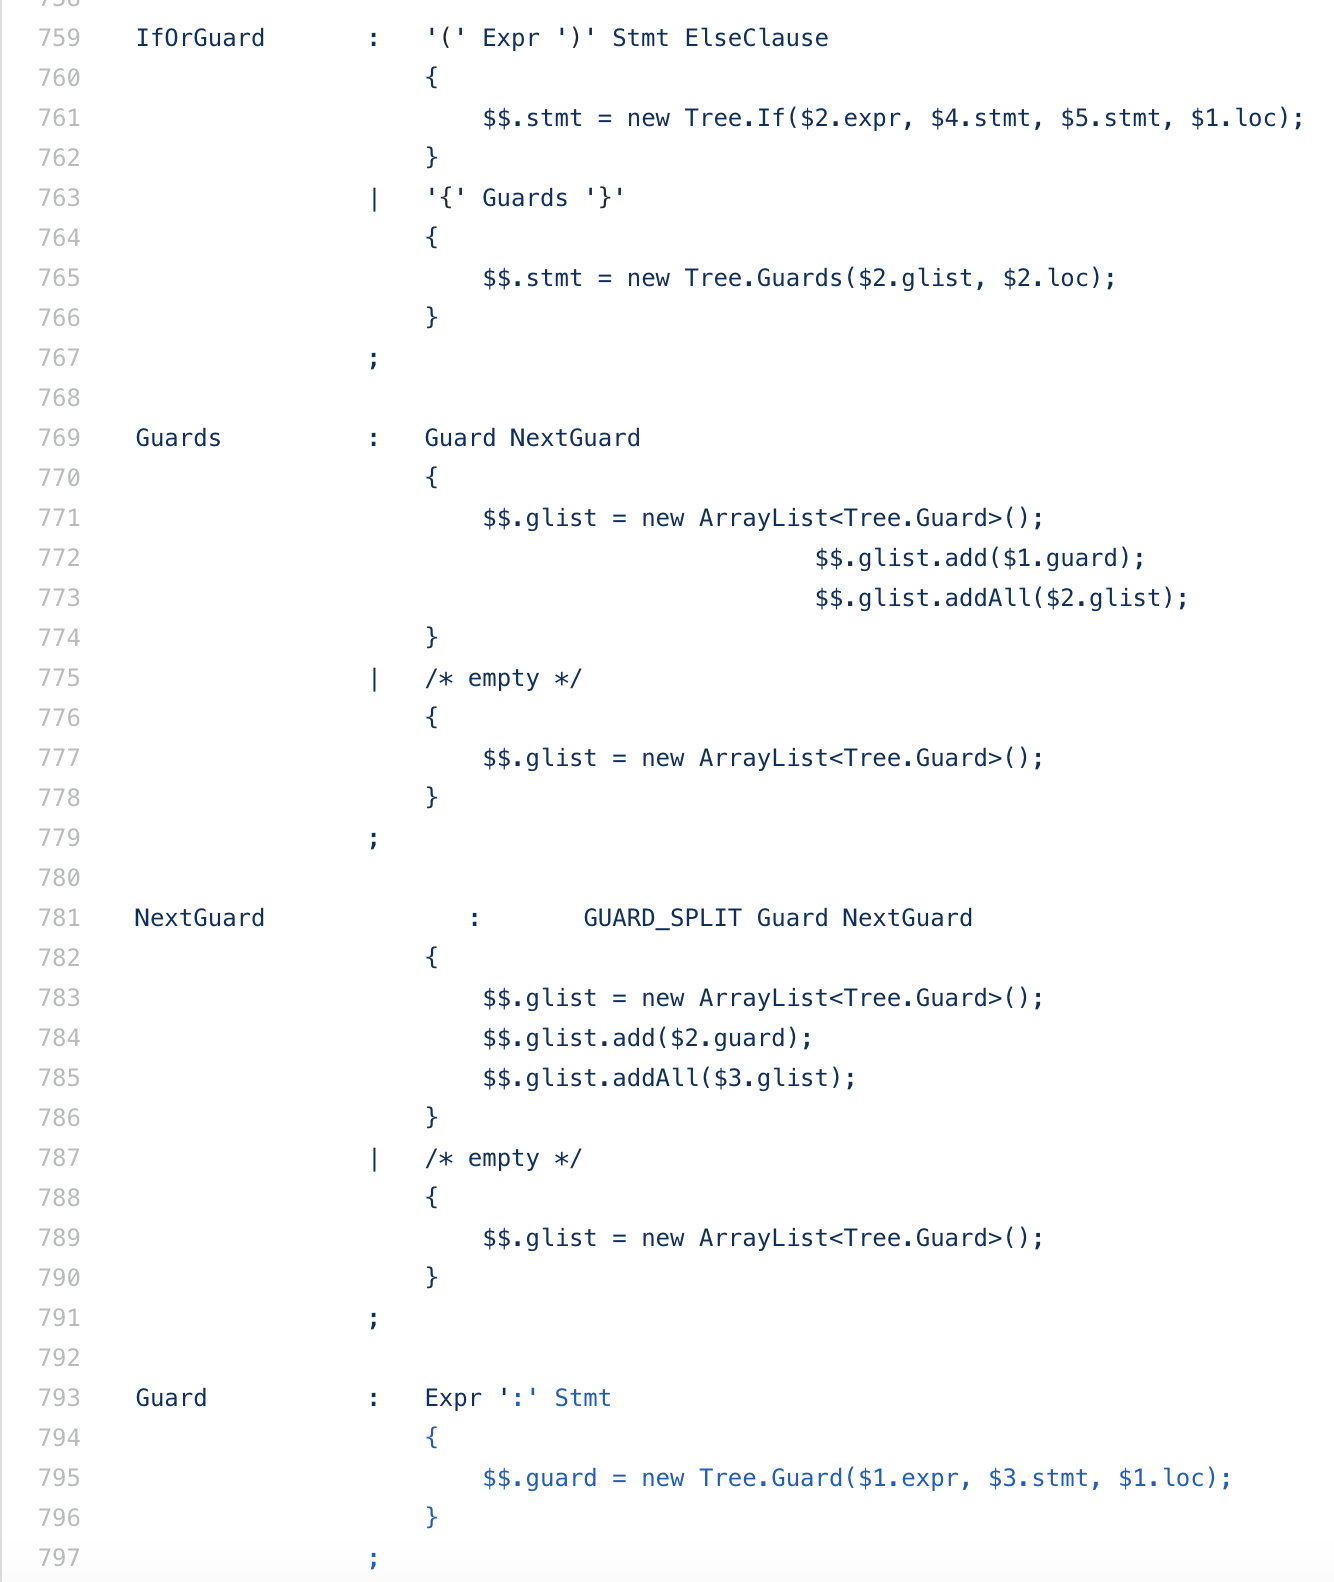
\includegraphics[width=5in]{guard.png}

    为了避免预测集有重合,Guard语法形如$Guards \to Guard NextGuard | \epsilon, NextGuard \to Guard NextGuard | \epsilon$

    注意语法规则描述里面还有另外一个问题是要解决和条件语句有公因子的问题。在代码中有所体现解决方案。

    \subsection{运算符优先级与左右结合}

    语法描述文件中已经告诉了如何解决优先级和左优先。其方法是令$Expr_k$表示优先级解析出来只有优先级高于等于$k$的运算符,用类似于$Expr_k = Expr_{k+1} <[+-] Expr_{k+1}>$ 这样的技巧来保证如果遇到优先级为$k$的运算符,那么一定不会被先解析,会先解析更高优先级的表达式$Expr_{k+1}$。

    左结合的实现是通过把$Expr_k$在解析的时候没有解析完的话不直接计算,而是存一个list,等到全部解析完之后再按照做结合计算得到一个表达式。右结合的话其实因为其本事是右递归,所以我们可以边解析边计算,最后得到的本身就是右结合。

    % 对于default 实现的时候,由于本身就和[符号一个优先级,其他运算符优先级都没他们高,所以这个时候直接用$Expr9[Expr] <default Expr_9>$就不太会出锅。

    \section{关于if不是严格LL(1)文法的问题}

    由于if(true) if(false) stmt; else stmt; 这句话可以被解释成两种不同的意思,根据wiki和生成的代码,pg会根据定义的规则顺序来给一个优先级。

    比如说$PS(ElseClause \to ELSE STMT)$ 和 $PS(ElseClause\to \epsilon)$里面是有共同的$else$,这个时候pg会根据定义的顺序,把else分配给第一个预测集。这样还是可以递归向下分析,而且是确定性的。

    \section{comprehension 表达式文法}

    如果这个时候简单的使用[,本身优先级和常量数组就一样。所以这个时候就需要处理公因子(或者预测集相同的情况)。但是,但是,如果下一个是LITERAL,我们无法判断这个是表达式还是常量,所以我们需要一个不含LITERAL 的表达式,和含LITERAL 的表达式,如果是LITERAL 还要再判断一步是不是for。

    \section{误报错误}

    \begin{lstlisting}
        class Main {
            static void main() {
                int[] xs;
                xs = [1,0,-1]; // -1 is an expression, not a constant!
            }
        }
    \end{lstlisting}

    这一段代码会爆两个错误,第一处在-1,第二处在]。此处再次感谢Harry Chen 提供思路。报两处错误的原因是当分析到-时候,爆第一次错误。这个时候由于$- \in Follow(Expr_5)$,所以会一路退出到分析表达式的那一步。这个时候识别成减法,接下来分析到]会再次出错。

    \end{document}